Рассмотрим случай n поставщиков, в котором все игроки максимизируют прибыль и осведомлены о значениях базовой функции друг друга при фиксированном бюджете $K_0$. Для удобства пронумеруем игроков по возрастанию значению базовой функции $P_i$. Таким образом $P_1 \le P_2 \le \dots \le P_n$.

Заметим, что в заданных условиях игрок $n$ может быть уверен, что при выставлении скидки $M_{n} >P_{n-1}$ он гарантированно выиграет аукцион. Тем не менее в целях максимизации математического ожидания прибыли он может быть заинтересован в выставлении меньшей скидки.

Игрок $n$ обладает информацией о базовой функции прочих игроков, но не знает об их стратегиях выставления скидки. В условиях независимого принятия решения игроками вероятность победы в закупке $p(\Delta M_n > \Delta M_i) (i = 1, … (n-1))$ при $M_n \le P_i$ равна $\Delta M_n/P_i$,  
то игрок $i$ c равной вероятностью выставляет скидку в меру своей базовой функции $Pi$, и $1$ при $\Delta M_nP_i$, конкурирующий поставщик не станет заключать сделку с отрицательной прибылью.

\begin{figure}[h]
	\centering
	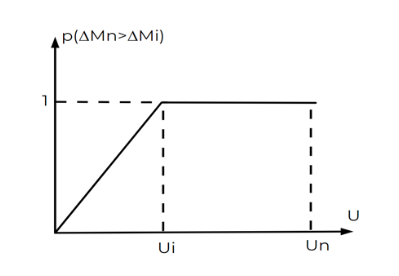
\includegraphics[width=0.5\textwidth]{assets/settings/probability_sale.excalidraw.png}
	\caption{Вероятность предоставить для поставщика n большую скидку чем конкурент $i$}
\end{figure}
Следовательно, математическое ожидание прибыли игрока $n$ в введенных обозначениях запишется как:
\begin{equation}
	\mathrm{E} n(\Delta M_n) =(Pn-\Delta M_n)p(\Delta M_n>\Delta M_1,\dots,n-1)=
\end{equation}
\begin{equation}
	=(Pn-\Delta M_n)p(\Delta M_n >\Delta M_1)...p(\Delta M_n >\Delta M_n-1) 
\end{equation}


\begin{figure}[h]
    \centering
    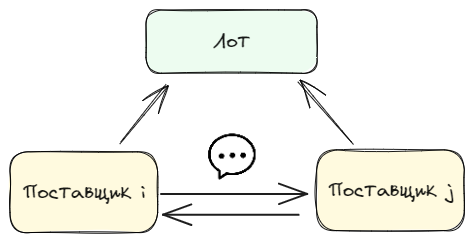
\includegraphics[width=0.5\textwidth]{assets/settings/collusion.excalidraw.png}
    \caption{Нежелательное поведение. Cговор}
\end{figure}

Полученная функция непрерывна, но не является гладкой от $\Delta M_n$. Имеются точки разрыва производных при значениях аргумента равных $P_i$.

Предложим алгоритм поиска оптимальной скидки $\Delta M_n$ для игрока $n$. Разделим поиск на два логических этапа:

1. Определяем аргументы, соответствующие условному максимуму, на каждом из интервалов гладкости. 

На интервале $\Delta M_n \in ( P_{i-1},P_i), (i = 1, … (n-1), P_0=0)$ математическое ожидание прибыли запишется как:
\begin{equation}
	E_n =(P_n-\Delta M_n)\frac{\Delta M_n}{P_i} \dots \frac{\Delta M_n}{P_{n-1}}\cdot
\end{equation}	
Оптимальное значение скидки соответствует условному локальному экстремуму на множестве $\Delta M_n \in (P_{i-1},P_i)$. 

Выполняем дифференцирование по $\Delta M_n$ правой части уравнения (3.9) и определяем максимум на интервале:
\begin{equation}
	\begin{aligned}
		& \Delta M_n^{(i)} =\text{arg} \max_{M_n} E_n \pi_n = \frac{P_{n}(n-i)}{n-i+1},\ \text{при} P_i> \frac{P_n(n-i)}{n-i+1}> P_{i-1}, \\ 
		& \Delta M_n^{(i)}=P_{i-1},\  \text{при} \ \frac{P_{n}(n-i)}{n-i+1} < P_{i-1}, \\
		& \Delta M_n^{(i)}=P_i , \ \text{при} \ P_i> \frac{P_n(n-i)}{n-i+1}
	\end{aligned}
\end{equation}

2. Находим оптимальное значение  путем нахождения максимума конечного числа локальных максимумов. Оптимальное значение скидки $\Delta M_n^{(opt)}$ задается как:
\begin{equation}
	\Delta M_n^{(opt)}= \text{arg} \max_{\Delta M_n^{(1)},\dots,\Delta M_n^{(n)}}\mathrm{E} \pi_{n} \cdot
\end{equation}
Заметим, что оптимальный вид скидки $\Delta M_n^{(opt)}$ в случае полной информированности будет определяться не только значением базовой функции поставщика $P_n$, но и соотношением между $P_1,\dots,P_n$.

Опишем применение алгоритма для игрока $i$. Вероятность победы в закупке игрока $i$ задается как:
\begin{equation}
	\begin{cases}
		p(\Delta M_i > \Delta M_j)= \frac{\Delta M_i}{Pj}, \ если \ i<j \\ 
		p(\Delta M_i >\Delta M_j)= \frac{\Delta Mi}{Pj}, \ при \ M_i<P_j \ и \ p(\Delta M_i > \Delta M_j)=1 \ при \Delta M_i \ge Pj, \  если \ i >j
	\end{cases}
\end{equation}
 
Аналогично математическое ожидание прибыли игрока i запишется как:
\begin{equation}
	E\pi_{i}(\Delta M_i) =(Pi-\Delta M_i)p(\Delta M_i>\Delta M_1, \dots ,M_{i-1},M_{i+1},..,M_n)=
\end{equation}
\begin{equation}
	=(P_i-\Delta M_i)p(\Delta M_i >\Delta M_1) \dots p(\Delta M_i >\Delta M_n) \cdot   
\end{equation}

$E\pi_{i}(\Delta M_i)$ имеет точки разрыва производных в $P_1,\dots,P_{i-1}$. Шаги оптимизационного алгоритма для игрока $i$ аналогичны поставщику $n$. На первом этапе выделяются максимумы на интервалах гладкости $M_i \in (0,P_1) ,(P_1,P_2) ,\dots,(P_{i-1},P_i)$. 
На втором выполняется поиск оптимального решения по конечному набору локальных максимумов, полученных на шаге 1: 
\begin{equation}
	\Delta M_i^{(opt)}= \text{arg} \max_{\Delta M^{(1)}i,\dots,\Delta M^{(i-1)}_i}  \mathrm{E}\pi_{i} \cdot 
\end{equation}

Подробно разберём случай двух игроков для интерпретации результатов. Игрок с большим значением базовой функции получит номер 2 и задаст скидку:
\begin{equation}
	M_1=P_1/2 , при P_1/2 < P_2 , \text{иначе} \ \Delta M_1=P_2 
\end{equation}

То есть в условиях максимизации прибыли и достаточно конкурентных игроков имеем случай аналогичный закрытому аукциону. Если поставщик обладает значительным преимуществом, то выставляет скидку равную значению базовой функции более слабого конкурента.

Обратим внимание, что в текущей постановке задачи поставщики предполагали стратегию прочих игроков неизвестной. При максимизации выигрыша в наихудшей из возможных ситуаций получаем тривиальный вывод, что поставщик $n$ предоставит скидку $P_{n-1}$, таким образом упуская выгоду от более рискованного предложения. 
